\documentclass{article}
\usepackage{graphicx}

\begin{document}
\title{Applying Information Theory to a Fully Recurrent Neural Network}
\author{Stefan Ivanovic, Vignesh Muruganantham, Benjamin Kha}
\date{April 23 2018}
\maketitle{}

\section{Abstract}

In this paper, we use information theory to analyze a fully recurrent neural network. The neural network is trained to predict daily temperatures from weather data in the past several days. We analyze if a natural structure develops in the network (since there is very little structure imposed on a fully recurrent neural network). To do this, we form graphs of the information flow in the network and develop an ranking algorithm to help analyze it�s structure. We find only slight traces of a structure developing on the network. We also analyze how information theory related statistics can be used as learning indicators. Additionally, we look at whether the information bottleneck principle appears to apply to fully recurrent neural networks (as it has been shown to apply to feed forward neural networks).  We find no indication that the information bottleneck principle still applies. 

\section{Background and Related Work}

Information theory has been a very successful tool for understanding neural networks. One important example of this is the application of the information bottleneck principle to feed forward neural networks. In �Opening the black box of Deep Neural Networks via Information� the mutual information between each layer of their feed forward neural network and the inputs and ground truth outputs were calculated. This showed that during training was split into two phases. In the first phase, the mutual information with the input and output both increased as one would naturally expect. In the second phase, the mutual information with the input significantly decreases and the mutual information with the output slightly decreased. In their paper, they described this second phase as learning to forget information about the input, in order to become more general. This relates to the information bottleneck principle, since the network appears to be �trying� to become like the �perfect� network which keeps the minimal information about the input which is sufficient for predicting the output. 
In the paper �Information Theory for Analyzing Neural Networks�, information theory was applied to recurrent neural networks; However, it was done on a very small toy network. Additionally, the analysis done was specifically fit to a very simple controller network. In this paper, we analyze the structure of a larger (than their toy example) fully recurrent neural network, designed for weather prediction.

\section{Creating the Information Flow Graph}

Our goal in creating a mutual information flow graph is to create a graph with neurons as vertices, and directed edges which best represent how information flows from each neuron to the next. The most obvious approach is to just calculate the mutual information between each neurons, and to create an edge connecting two neurons if this mutual information is above some cut off. However, this has multiple problems. The most obvious problem is that this would create an undirected graph, however, that can be fixed by just replacing regular mutual information with time delayed mutual information. The greater flaw is that this would create false edges representing incorrect information flow. This is best explained through an example. If neuron A greatly  influences neuron B and neuron C, then their will be a high mutual information between B and C because they both have a high mutual information with A. Therefore, using mutual information directly would produce an edge between B and C, despite the fact that no information flows between B and C. Using time delayed mutual information technically fixes this problem, however, it also has similar problems (which require slightly more complicated examples to show which will not go into). The solution is simply to look at the time delayed mutual information minus the mutual information, which we will define as the information flow rate between two neurons. This calculates how much each neuron directly influences the other neurons and removes the effect of two neurons having a high mutual information without actually influencing each other. 
 Using this method to calculate the information flow in the network, we develop the following chaotic information flow graphs. The difference between the graphs is just the cut-off point we choose for how high the information flow rate must be in order to add an edge to the graph.
 
 
 
 After doing some basic analysis of the graphs, we were not able to find any major patterns. However, we did see a negative correlation between the input degree and output degree. This indicates that some neurons provide information to many neurons and others absorb information from other neurons, but neurons rarely do both. The following plots show this negative correlation. 
 
 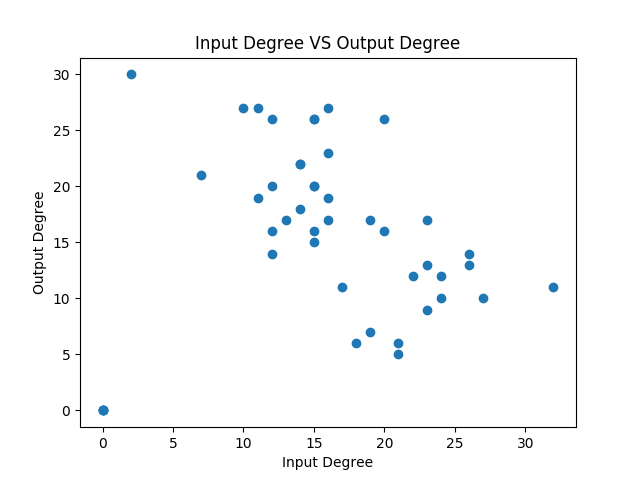
\includegraphics[width=\linewidth]{RNN_Images/6_006}
 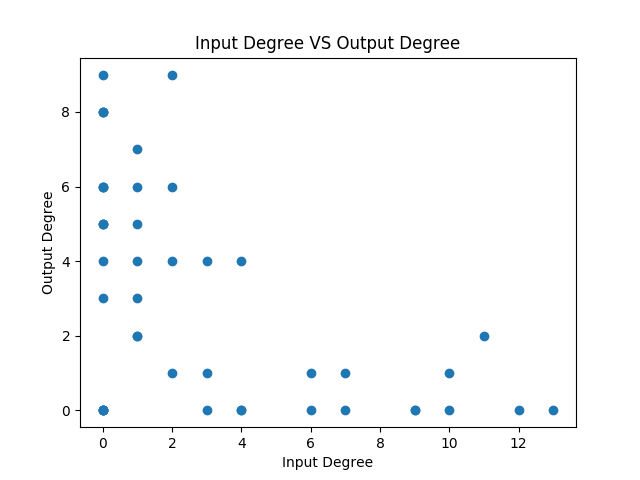
\includegraphics[width=\linewidth]{RNN_Images/4_03}
 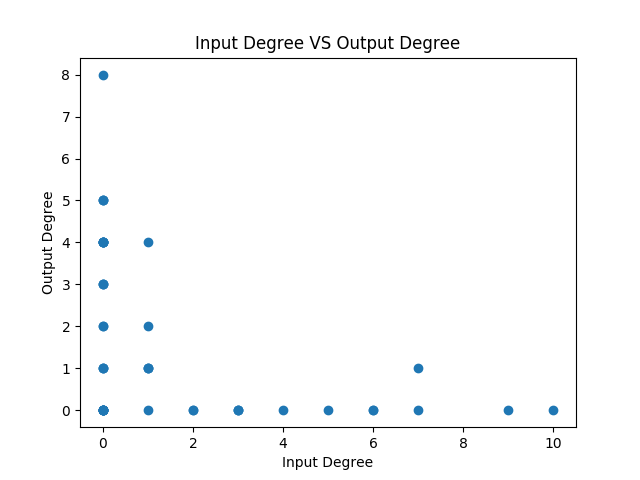
\includegraphics[width=\linewidth]{RNN_Images/5_04}

Additionally, we have the following degree histograms. These show a lack of any clear pattern in the degrees. 

 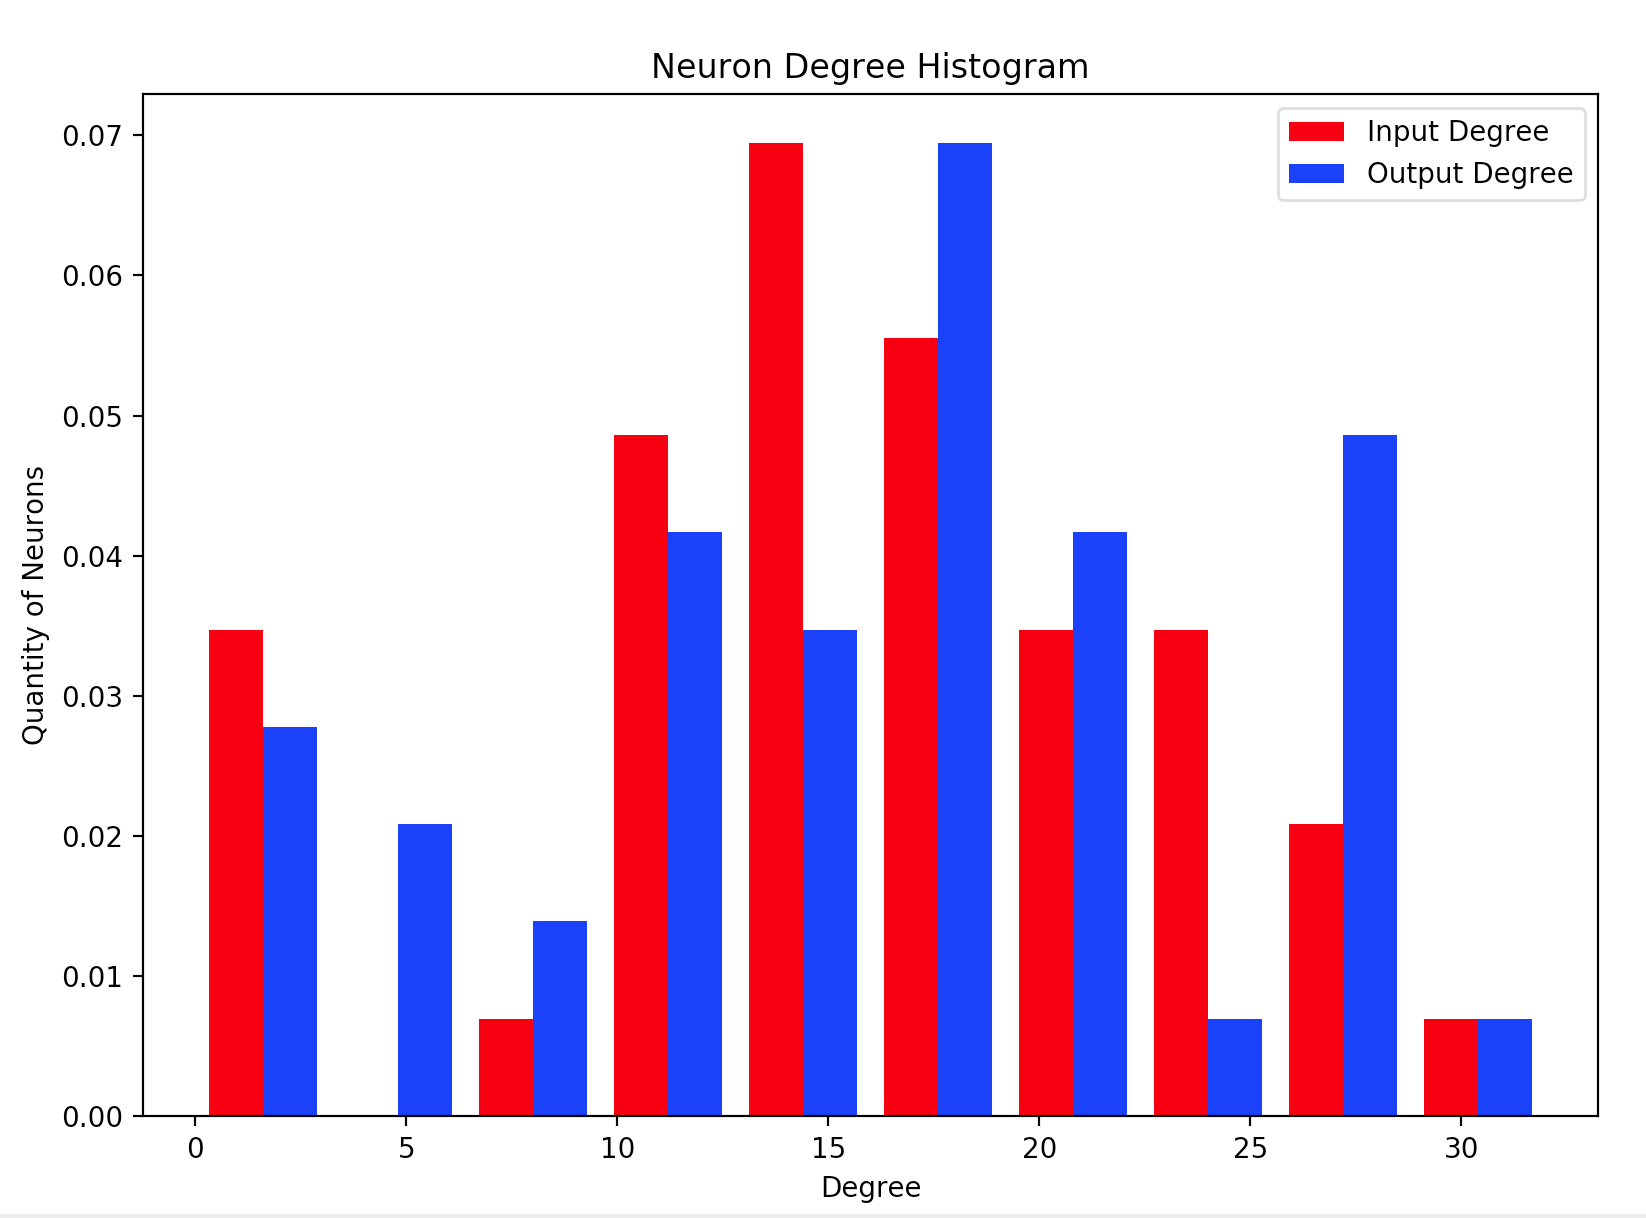
\includegraphics[width=\linewidth]{RNN_Images/3_CutOff006}
 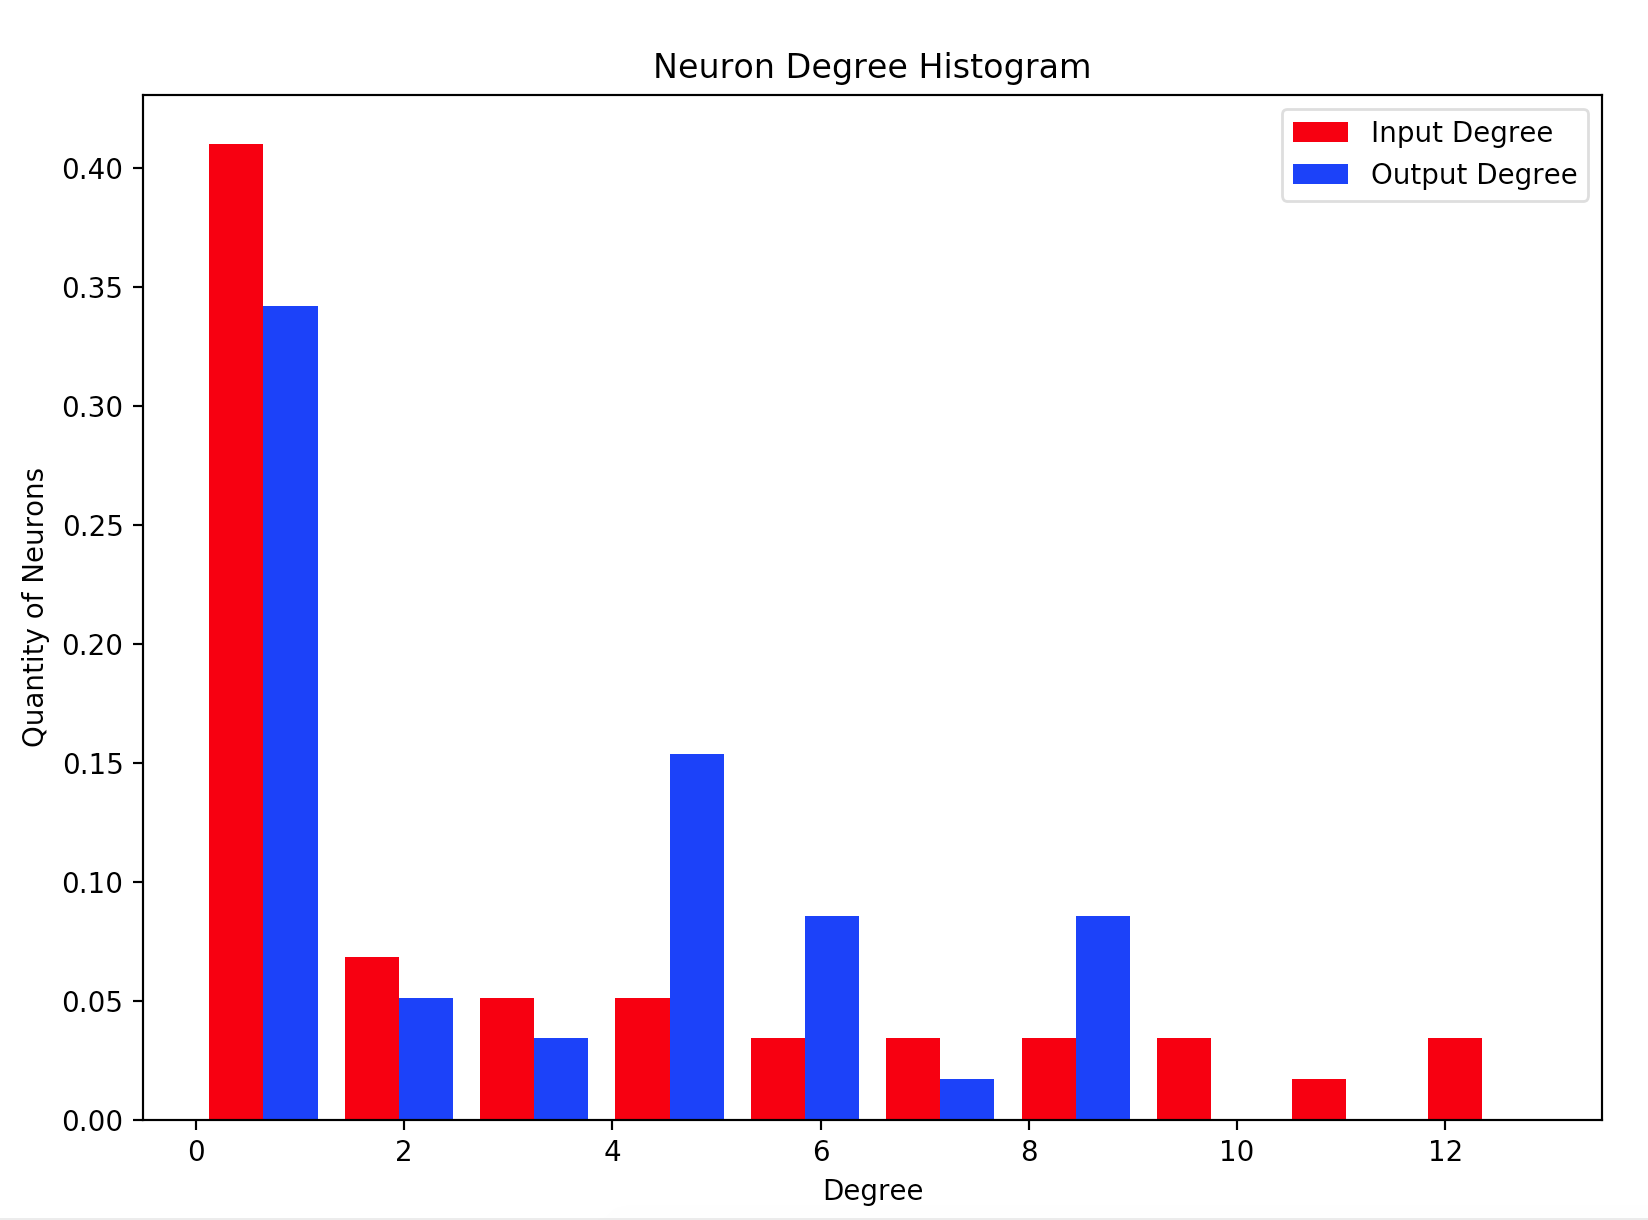
\includegraphics[width=\linewidth]{RNN_Images/2_CutOff03}
 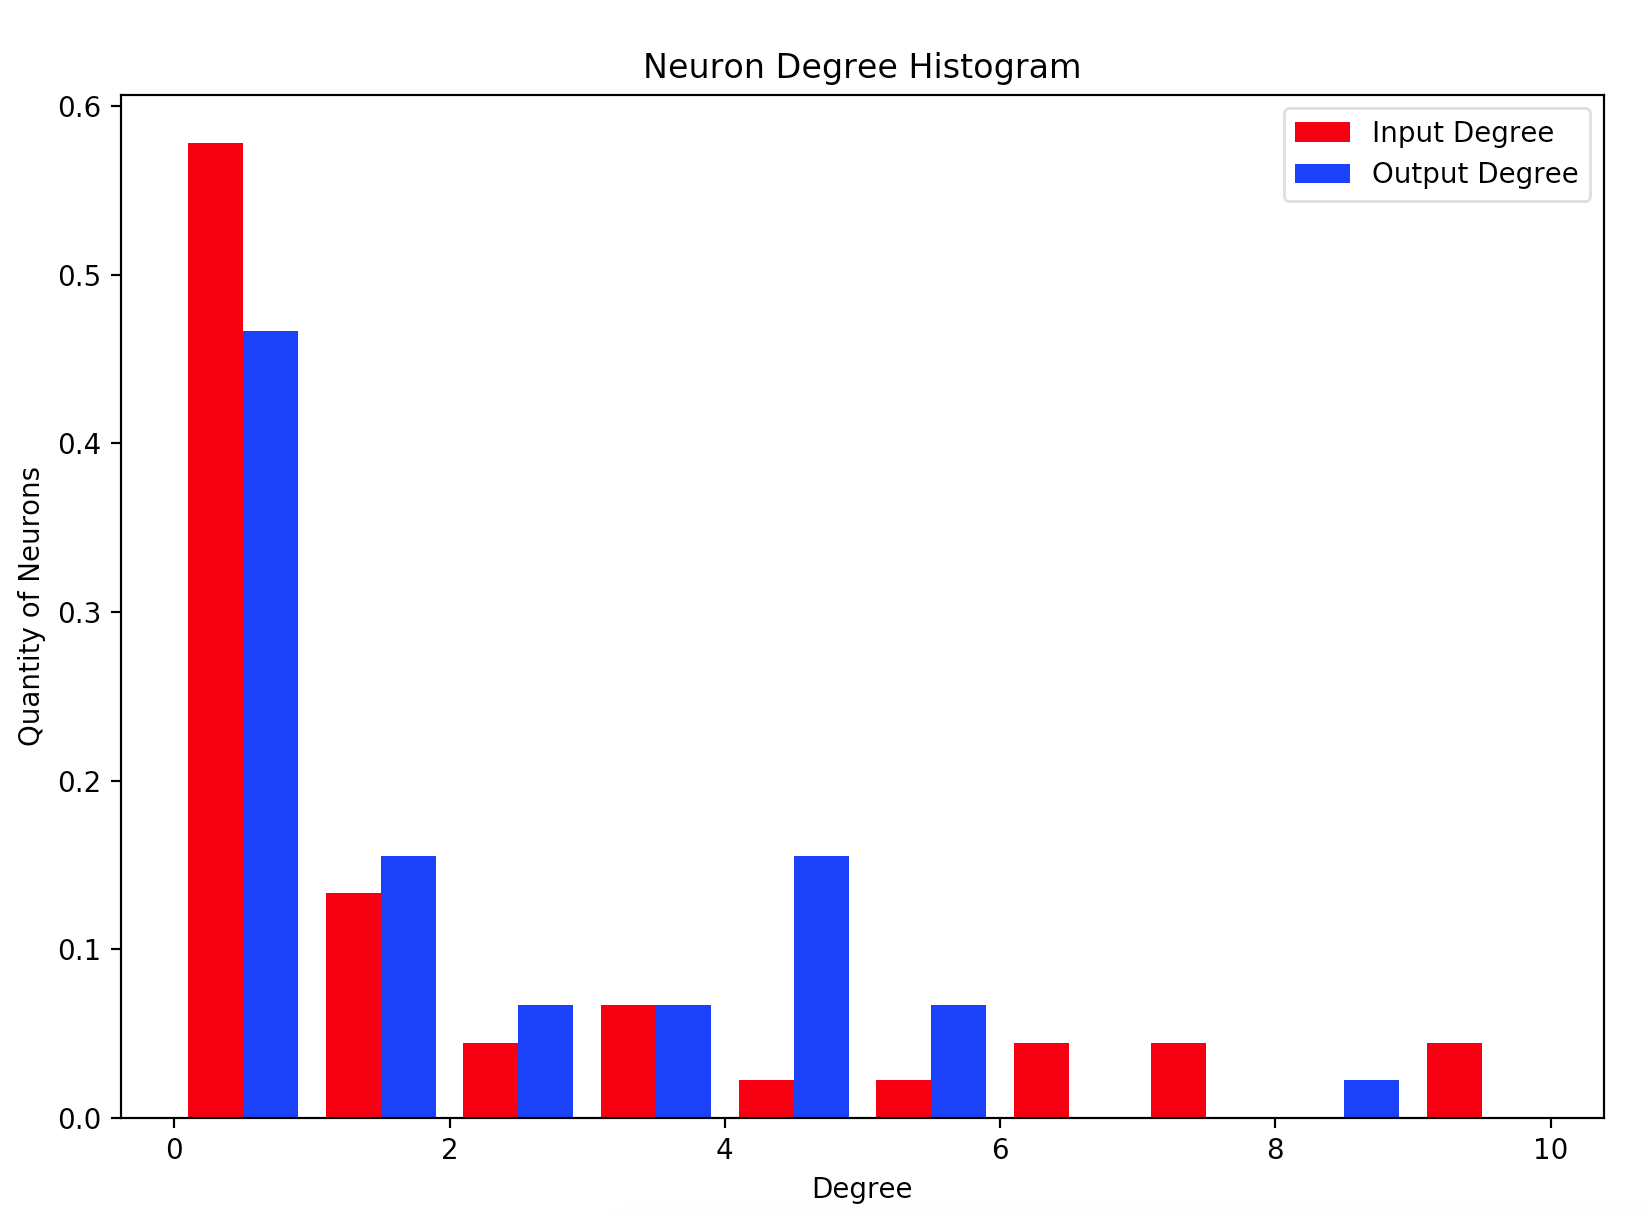
\includegraphics[width=\linewidth]{RNN_Images/1_CutOff04}
 
 \section{The Ranking Algorithm}
 
 The feature of fully recurrent neural network that separates them from feedforward neural networks is the ability for ever hidden neuron to send information to every other hidden neuron. This removes the natural ordering to the neurons (by layer) that ordinary feed forward neural networks have. Therefore, one of the most natural things to look for in the structure of our neural network is weather it naturally has an order to it, similar to the layers of a feed forward neural network. To do this, we must develop an ordering algorithm to determine an ordering on the neurons from the information flow graph. We say the rank of a neuron is a real number which represents how �far along� the network a certain neuron is. In a feed forward neural network, we expect the rank of the neuron to increase as the layer the neuron is in increases. We define a ranking of the neurons to be a list of ranks of all of the neurons. 

 Let $N = \{1, 2, 3, ... n\}$ indicate the set of neurons. Let $r_{i}$ denote the rank of the ith neuron. Let $E_{ij}$ be $1$ if their is an edge from $i$ to $j$ and $0$ otherwise. $E_{ij}$ indicates wether their is a high information flow rate from $i$ to $j$ or not. Let $I_{i} = \{ j \in N |\ E_{ji} = 1\}$, and $O_{i} = \{ j \in N |\ E_{ij} = 1\}$. $I_{i}$ is the set of neurons that send a high amount of information to $i$, and $O_{i}$ is the set of neurons that have a high amount of information sent from $i$. If our network was a feed forward network, we would ideally want the rank of a neuron to be the layer than neuron is in. Alternatively we could represent this desire by saying we ideally want $r_{i} = r_{j} + 1$ if $j$ is in the layer before $i$. The set $I_{i}$  of neurons which send information directly to $i$ should logically be a subset of the neurons in the layer before the layer $i$ is in, so we naturally want $r_{i} = r_{j} + 1$ if $j \in I_{i}$. Similarly, we want $r_{i} = r_{j} - 1$ if $j \in O_{i}$. Therefore, we want the following.
 $$r_{i} = \frac{1}{ | I_{i} | + |O_{i} |}(\sum_{j \in I_{i}} (r_{j} + 1) + \sum_{j \in O_{i}} (r_{j} - 1))$$
 
 We can define a re-ordering algorithm as taking the rankings of the neurons and recalculating them according to the above equation. Although we got our inspiration from feed forward neural networks, this applies very well to our fully recurrent neural network. We can then define our ranking algorithm as simply applying the re-ranking algorithm over and over again until the ranks converge. 
 
 Although we don't a priori have a ranking on our hidden neurons as we would with a feed forward neural network, we do know that logically, our inputs should be ranked before our hidden neurons which should be ranked before our output neurons. Seeing this result in our ranking calculations would provide very strong evidence that our information flow graph and ranking algorithm are accurate. We have the following histograms of the rankings of the inputs, hidden neurons, and outputs (with different information flow rate cut off points). 
 
 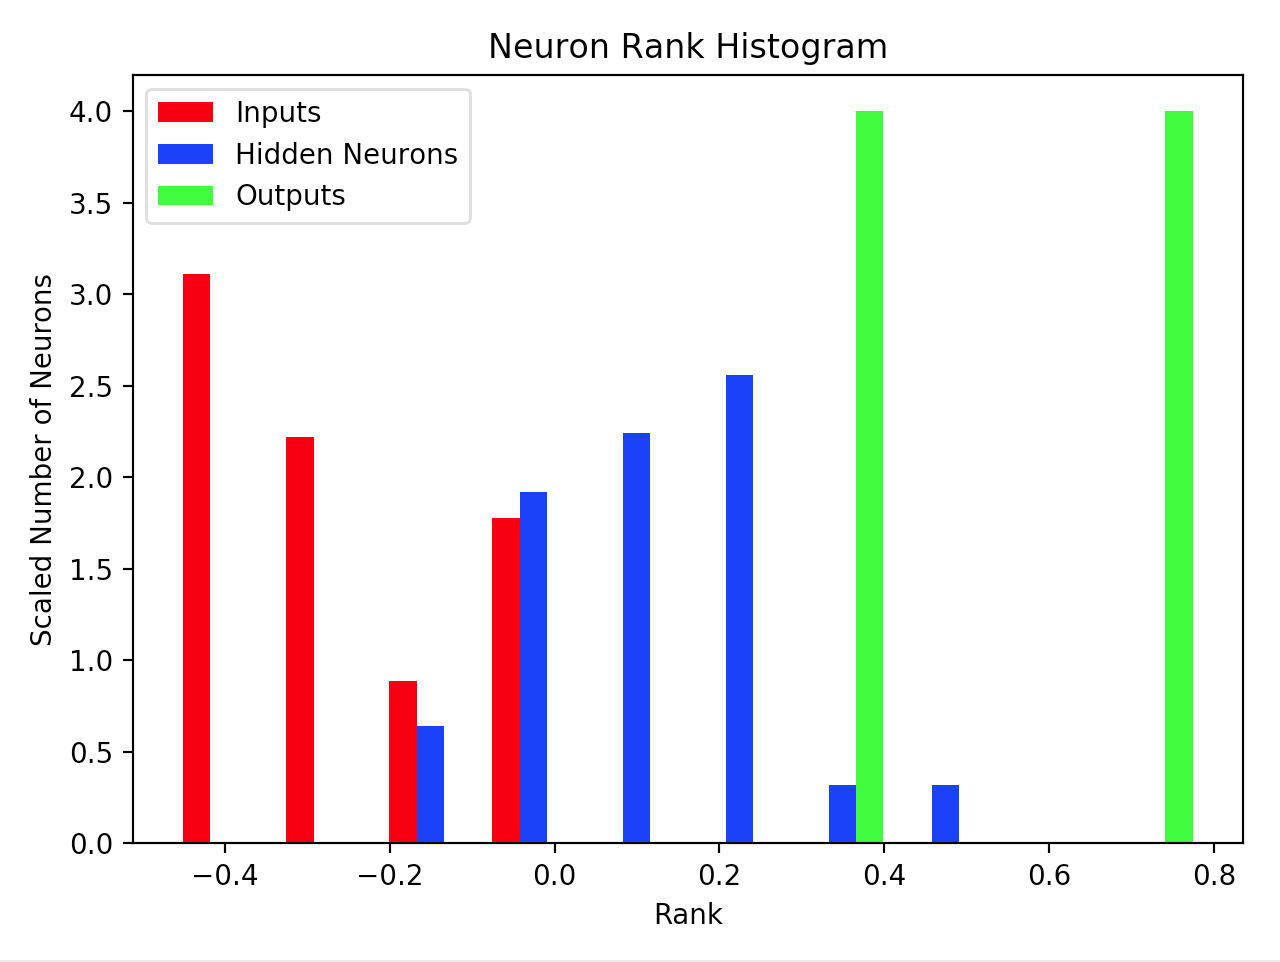
\includegraphics[width=\linewidth]{RNN_Images/22}
 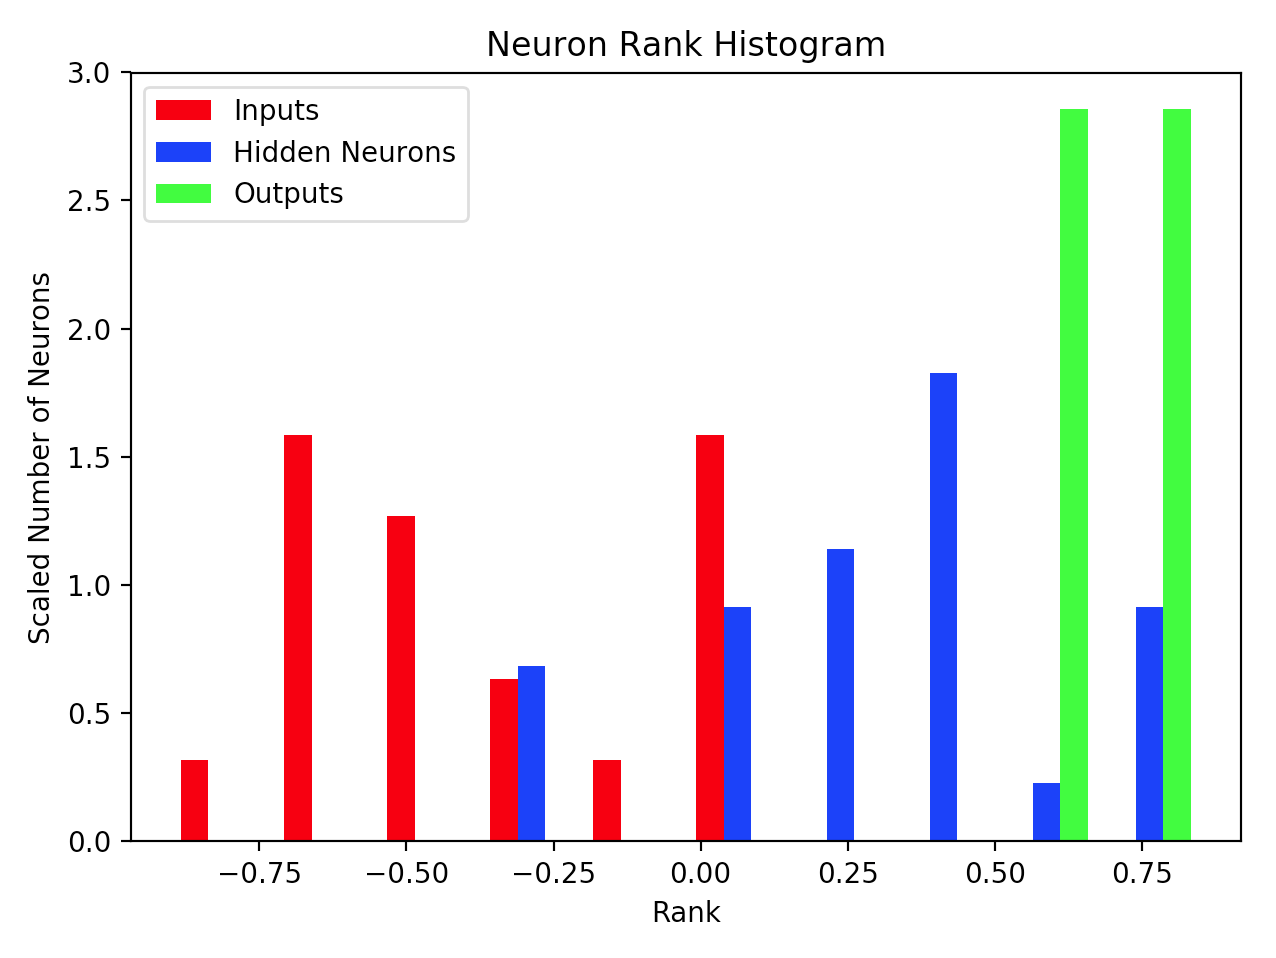
\includegraphics[width=\linewidth]{RNN_Images/23}
 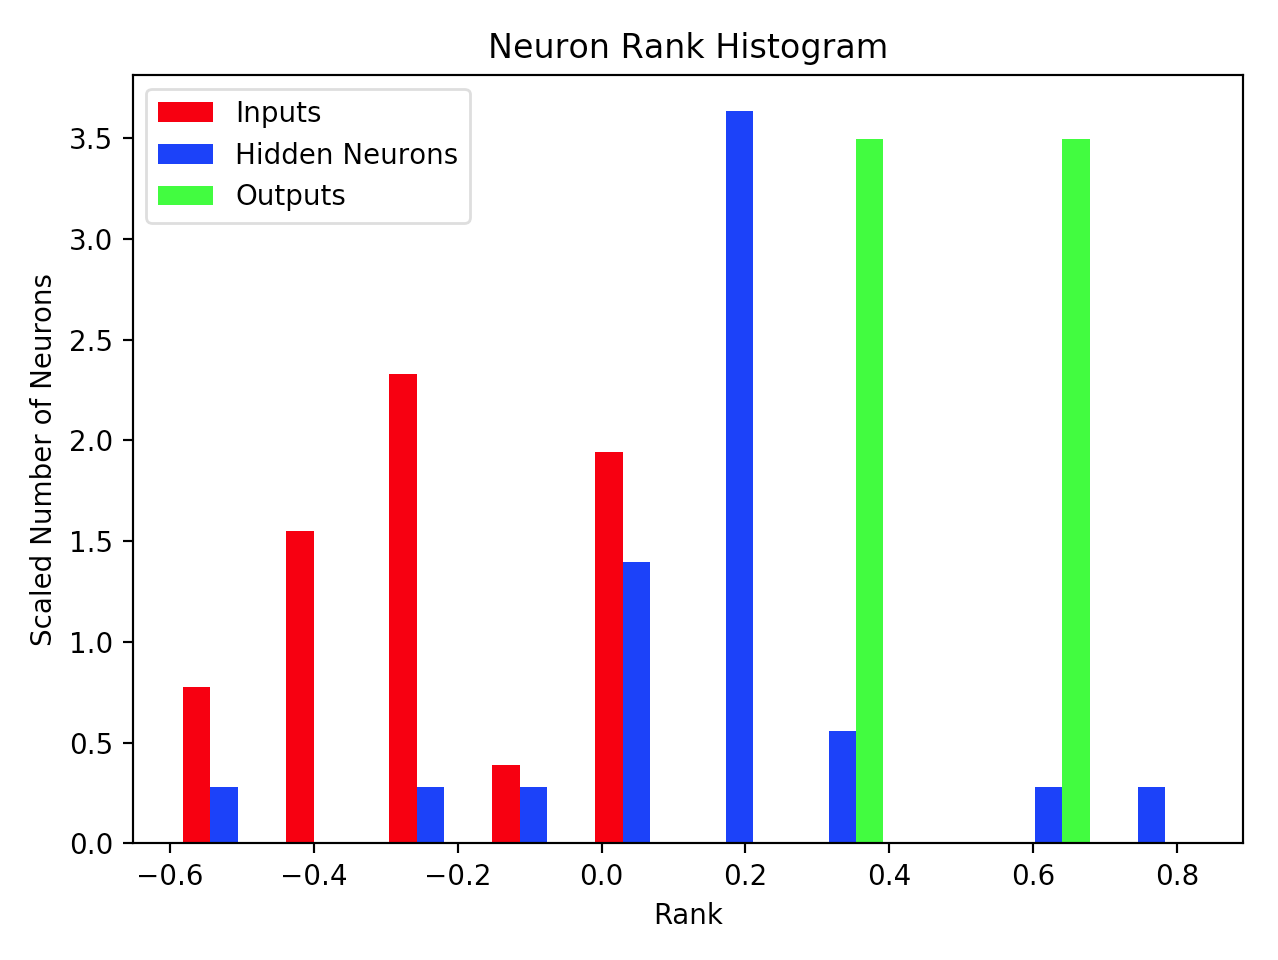
\includegraphics[width=\linewidth]{RNN_Images/24}
  
  Note, the algorithms not exactly ranking the inputs before the hidden neurons before the outputs is not always incorrect. For example, if we had the toy network with the connections Input $\rightarrow$ A $\rightarrow$ B $\rightarrow$ C $\rightarrow$ D $\rightarrow$ E $\rightarrow$ Output, and Input $\rightarrow$ F $\rightarrow$ Output, one could reasonably rank A before the input because it takes 5 steps to go from A to the Output, yet only 2 steps to go from the input to the output. This is only a toy example, however, it shows that a bit of "error" in ranking the inputs, outputs, and hidden neurons is not necessarily a bad thing. Aside from this, we do not see much interesting structure (or patterns) in the rankings. 
  
  \section{Input and Output Mutual Information During Testing}
  
  Another thing we can test to try to probe the natural structure of the network is looking at the mutual information of each neuron with the input layer and ground truth outputs during training. If we get a negative correlation between the mutual information with the input and mutual information with the output, this would show the neurons "forgetting" information about the inputs as they better fit the outputs. This would provide evidence for the information bottleneck principle applying to fully recurrent neural networks. However, this is not what we see. We will discuss why this is after showing the images, however, we do want to immediately note that is, by its self, is not evidence against the information bottleneck principle applying to fully recurrent neural networks. 
  
 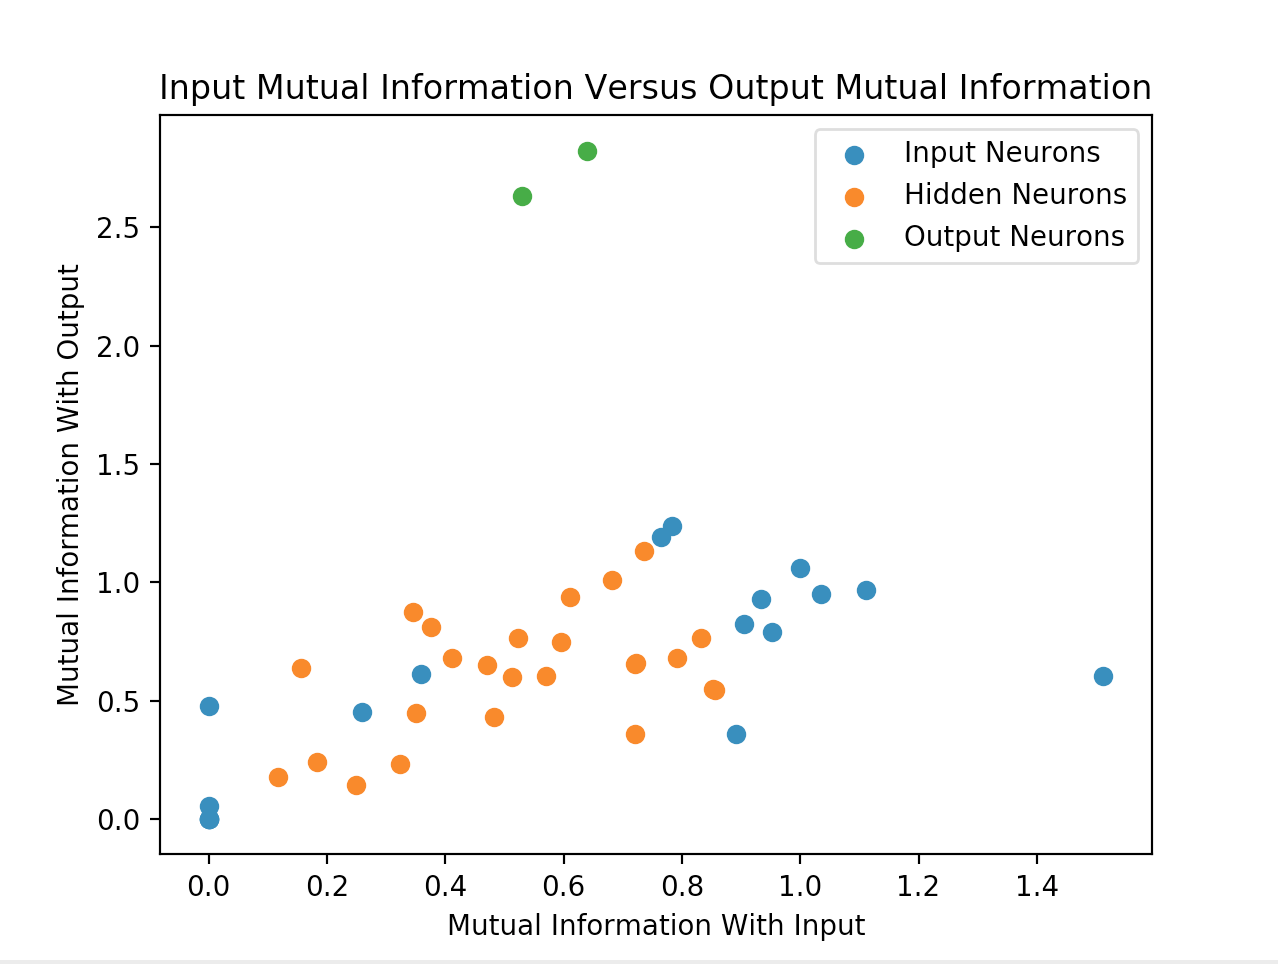
\includegraphics[width=\linewidth]{RNN_Images/11}
 
We see that the output neurons both have a correlation with the ground truth output, as expected. These two neurons do not reveal any interesting results, so we can remove them from the plot and get the following. 
 
 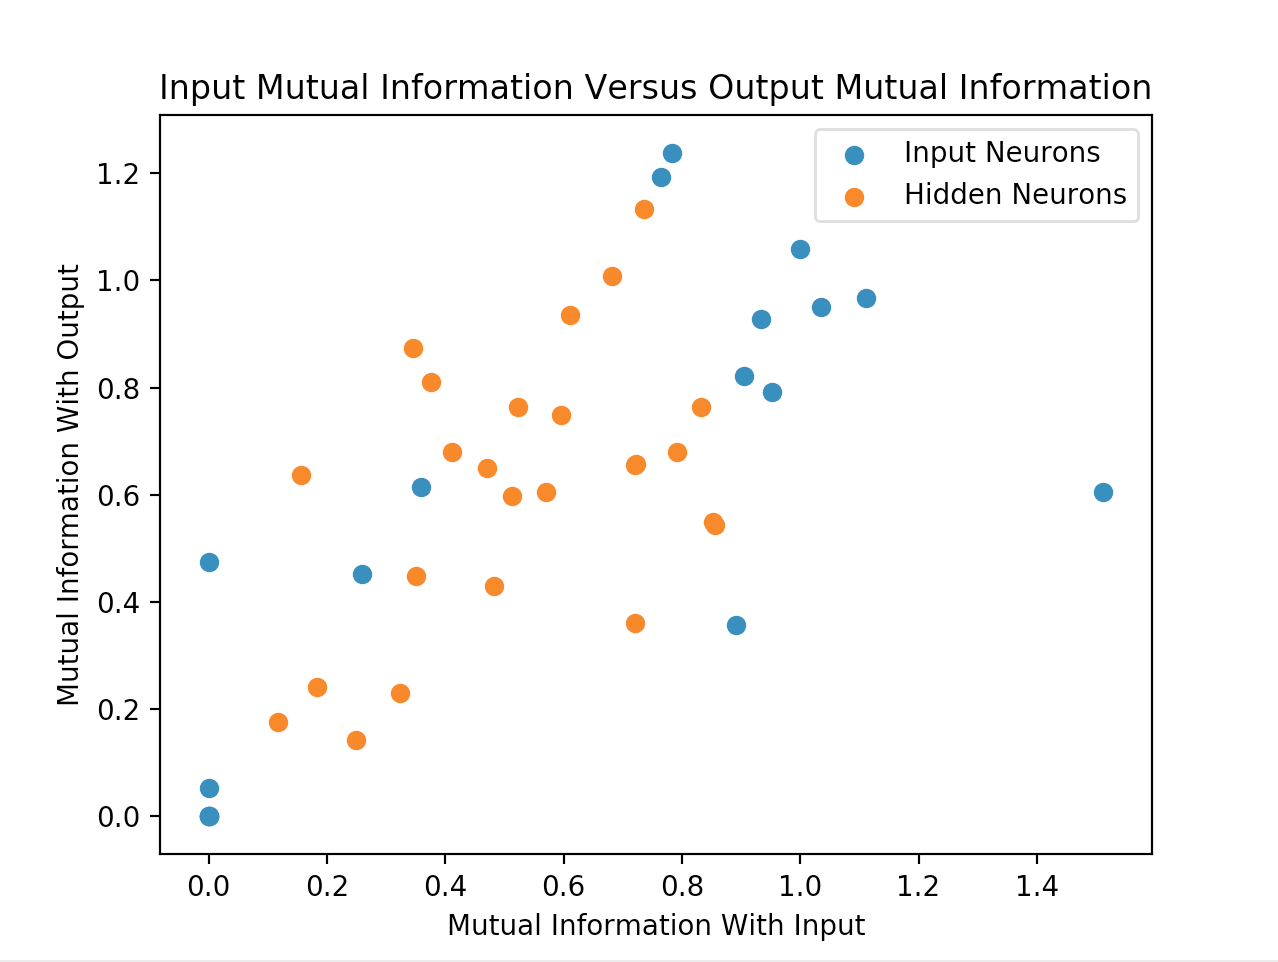
\includegraphics[width=\linewidth]{RNN_Images/10}
  
 There clearly appears to be a positive correlation between the mutual information with the inputs and the mutual information with the outputs. One might think that this could be caused by some neurons simply having more information than others. However, if we divide by the total amount of information (the entropy) of each neuron, we get the following plot.
 
 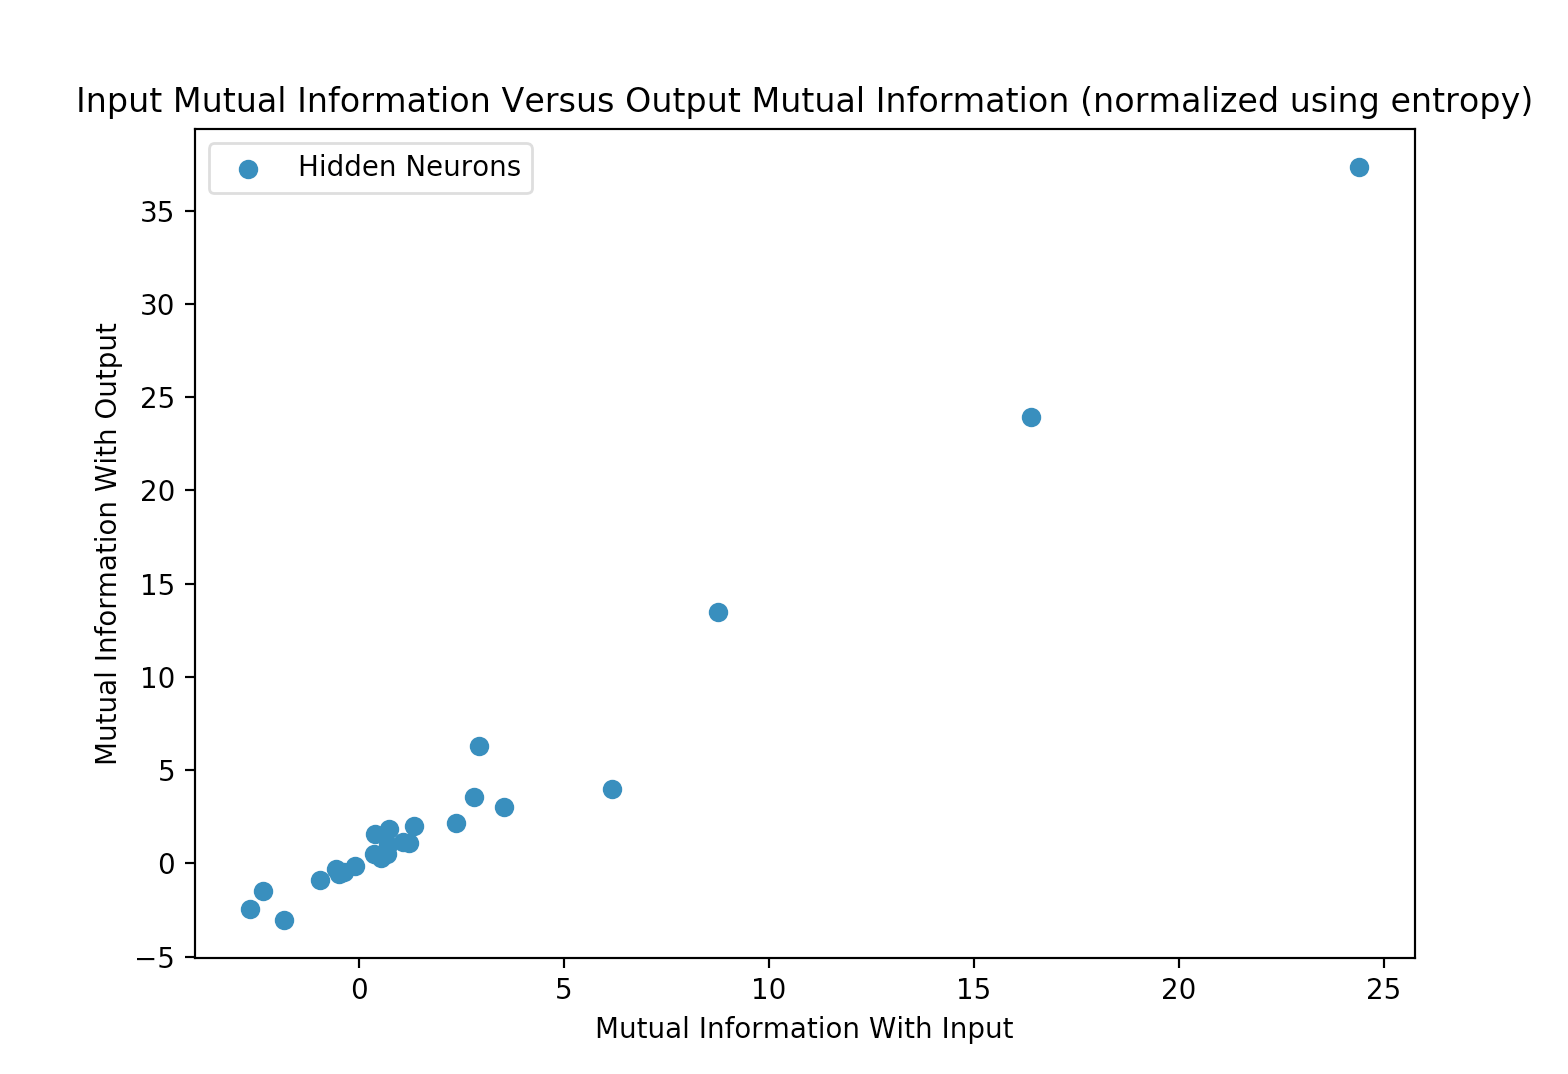
\includegraphics[width=\linewidth]{RNN_Images/12}
 
 This plot has an even higher positive correlation, so we can dismiss that possibility as the reason for the positive correlation. Note, we should not read too much into this increased positive correlation when dividing by the entropy , since this "positive correlation" is also what we would expect if the entropy was just a widely varying random variable. In my opinion, the most likely explanation for the positive correlation between the mutual information with the input and the mutual information with the output is just that some neurons are more important than others. The more important neurons then have a higher mutual information with both the input and the output. A very simple example where this could occur is if we are trying to replicate some function with multiple underlying processes. If some neurons are dedicates to each process, and not all the processes are equally important, this naturally results in widely varying neuron importance, in even an ideal network. It is very reasonable to expect this to be the case for our task (weather prediction). 
 
  \section{Input and Output Mutual Information During Training}
  
In addition to looking at the mutual information of the neurons with the inputs and ground truth outputs during testing, we can see how these values change during training. If we do this for each neuron in the hidden layer individually, the plot is very chaotic and hard to follow.
  
 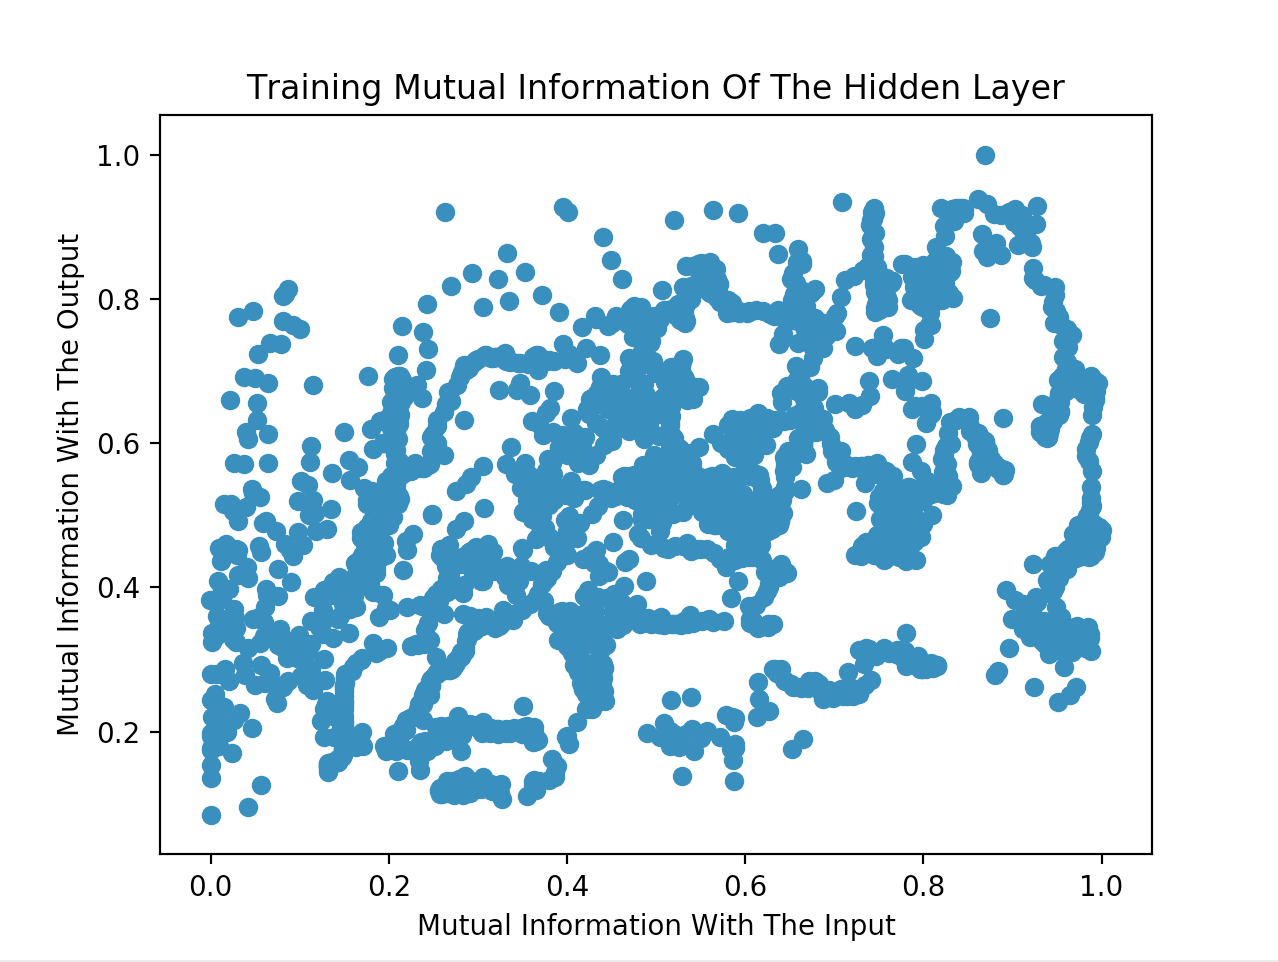
\includegraphics[width=\linewidth]{RNN_Images/17}
   
It is much nicer to look at the mutual information between the entire hidden layer and the inputs and ground truth outputs  This results in the following plot. We use a line plot instead of a scatter plot in order to help convey the order of the data points in terms of what time-step they are. 
 
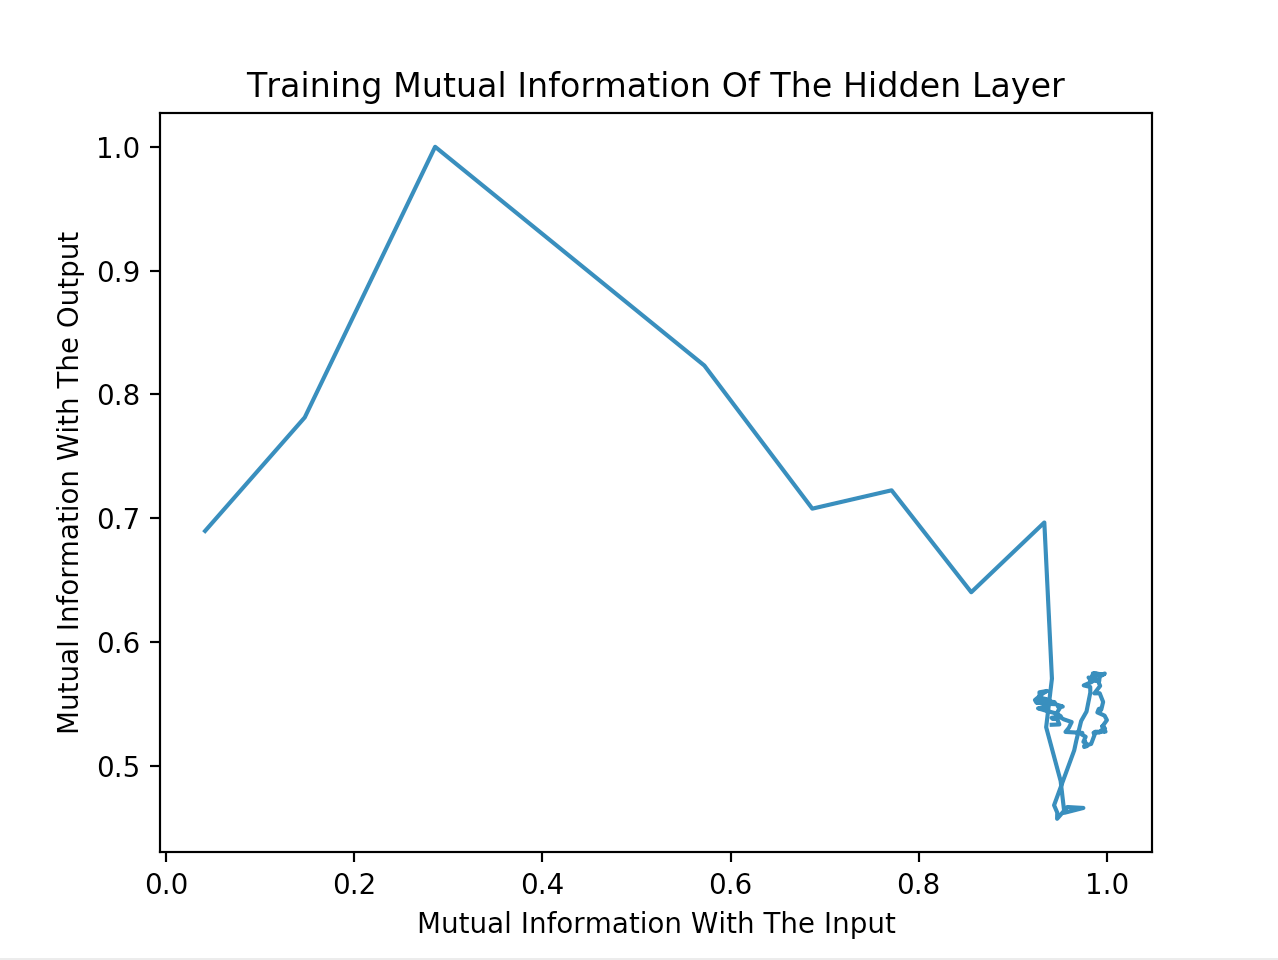
\includegraphics[width=\linewidth]{RNN_Images/13}
 
 If the information bottleneck principle applied to our fully recurrent neural network, we would expect the mutual information with the input to increase and then begin to decrease. We would also expect this to happen with the mutual information with the ground truth output, but to a much smaller extent. Instead, we only see the mutual information with the input increase (not decrease). We also see the mutual information with the output significantly increase, then decrease, then increase again. The learning does seem to be split into some phases, like how learning for feed forward neural networks can be split into two phases according to "Opening the black box of Deep Neural Networks via Information�, however, the phases are very different from feed forward neural networks. We were not able to come up with any theoretical justification to the phases of learning we see. Looking at the mutual information between the outputs (both the individual neurons and the layer as a whole) we get the following plots.
 
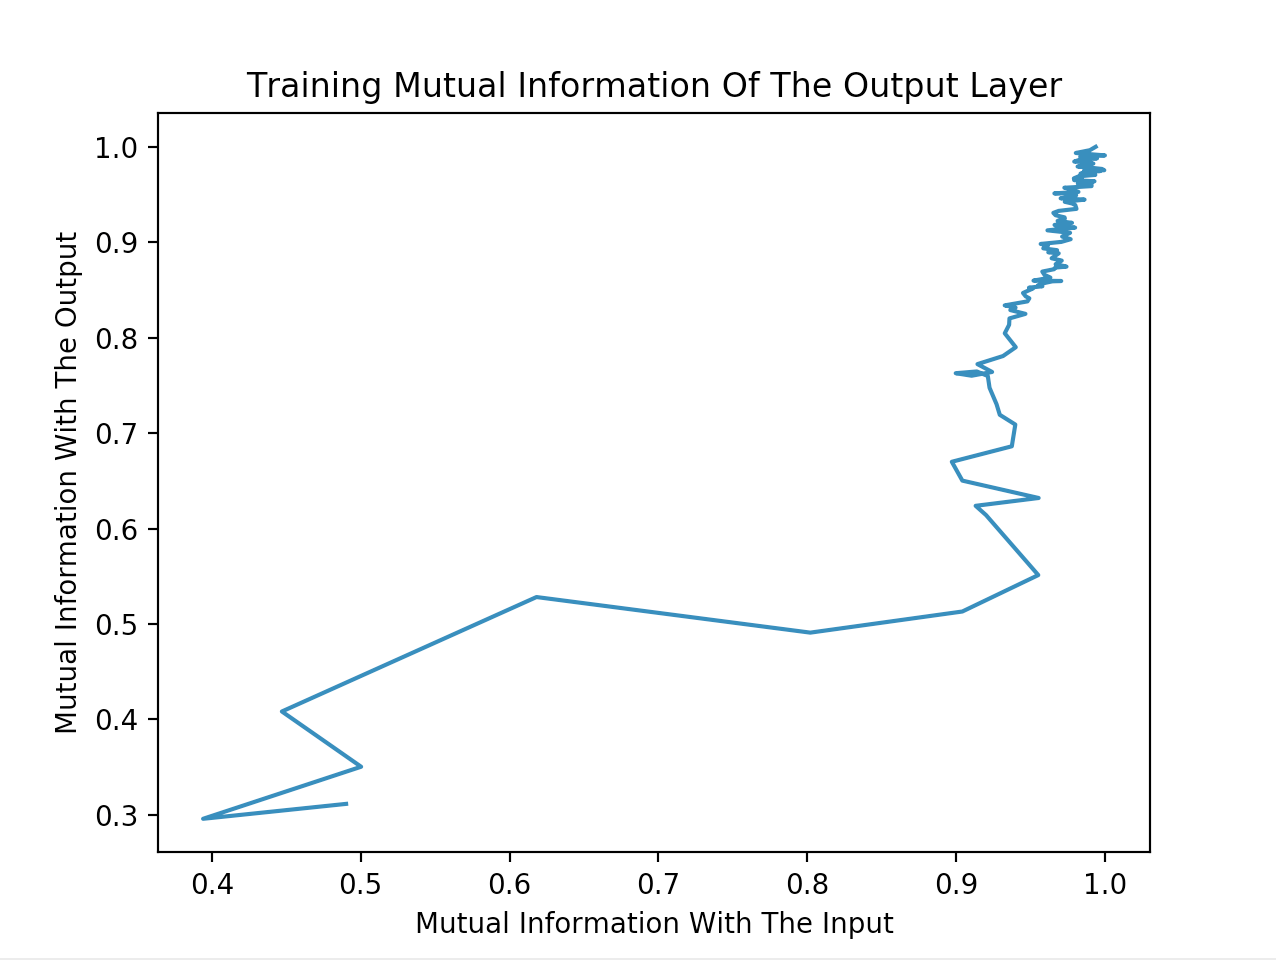
\includegraphics[width=\linewidth]{RNN_Images/14}
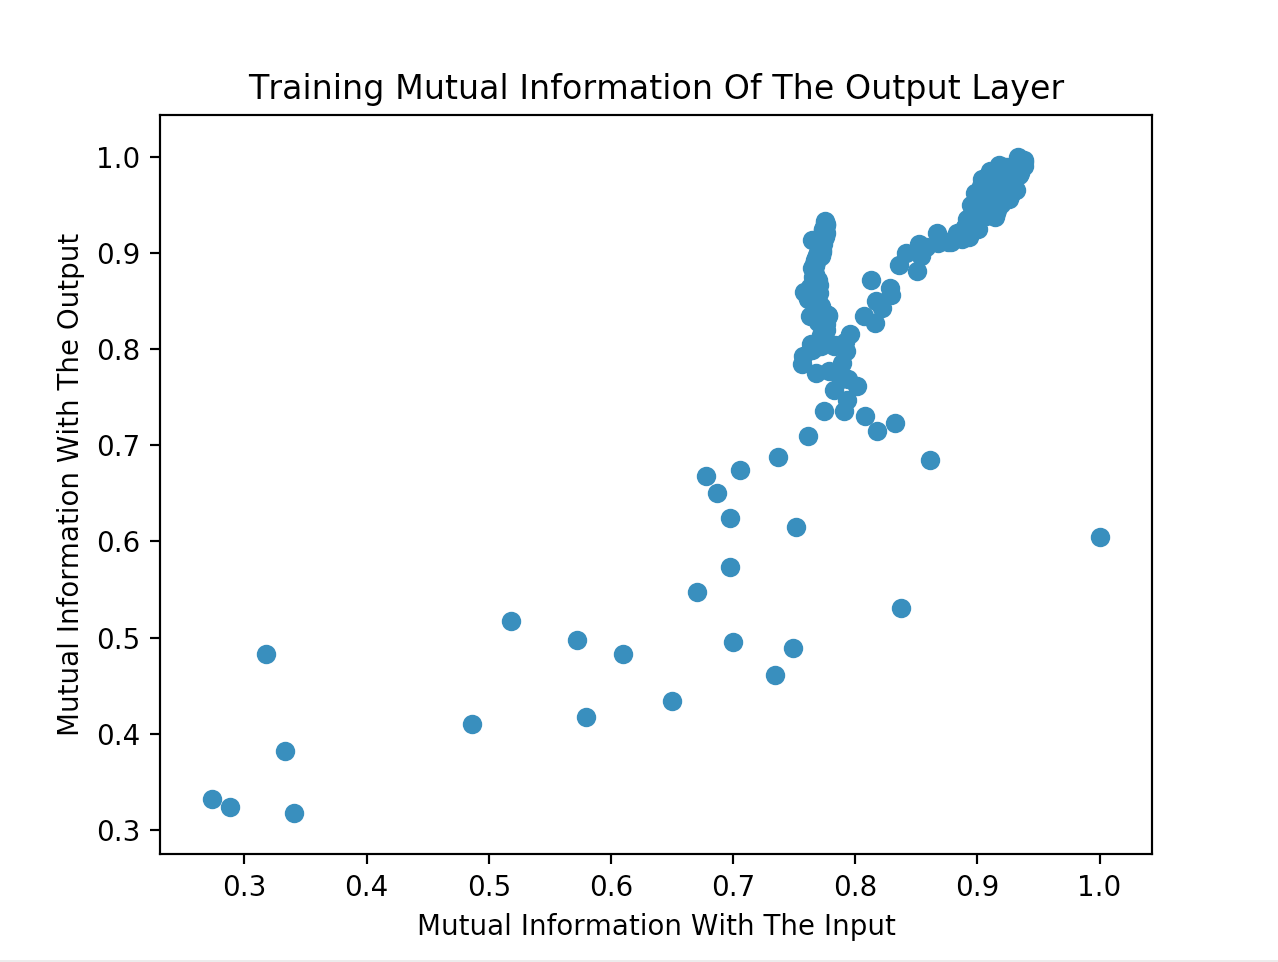
\includegraphics[width=\linewidth]{RNN_Images/15}
 
 Here we also do not see any indication of the information bottleneck principle applying. In fact, unlike with the hidden neurons, the mutual information with the ground truth outputs never decreases. The network just learns to use the information about the ground truth outputs stored in the hidden layer more efficiently. It is possible that the mutual information between the hidden neurons and the ground truth output decreases while the output layer learns to use that information more efficiently, and then begins to increase again once the information is being used as efficiently as feasible. However, that is purely a hypothesis, and we have no empirical evidence to support this idea. We created the following plot of the error and the mutual information of the hidden layer with the ground truth output both of the purpose to try to give more hints to understanding this phenomena. 

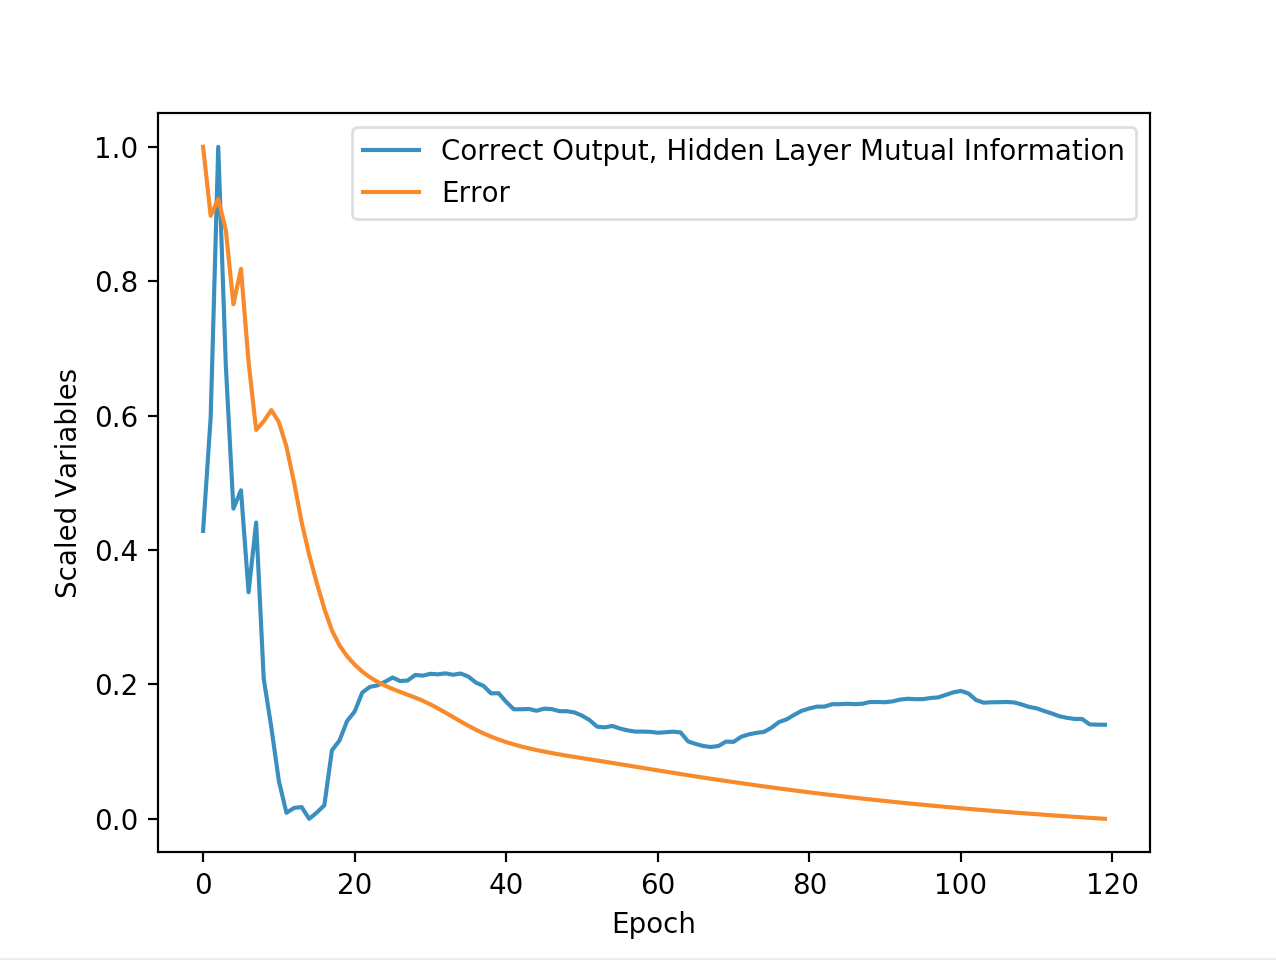
\includegraphics[width=\linewidth]{RNN_Images/20}
  
 The majority of the error decreasing appears to be happening as the mutual information with the ground truth output is decreasing (which is the opposite of what one would naturally expect); However, we have no evidence that this is not just a coincidence. Applying our analyses to other fully recurrent neural networks in the future could potentially help see if this is meaningful. 
 
 \section{An Analysis of Learning Indicators}
 
 In "Information Theory for Analyzing Neural Networks" it was shown that the mutual information of the neurons with the [NOTE: Ben and Vignesh look into this. I forgot if its mutual information with the output or mutual information with the input] is a useful learning indicator. This usefulness is primarily a result of the mutual information increasing before the error starts significantly decreasing. We test if we can replicate this result for a fully recurrent neural network, and test for other learning indicators. Mutual information between the output and the ground truth output almost perfectly mimics the (negative of) the error (as one would naturally expect) as in the following plot.
 
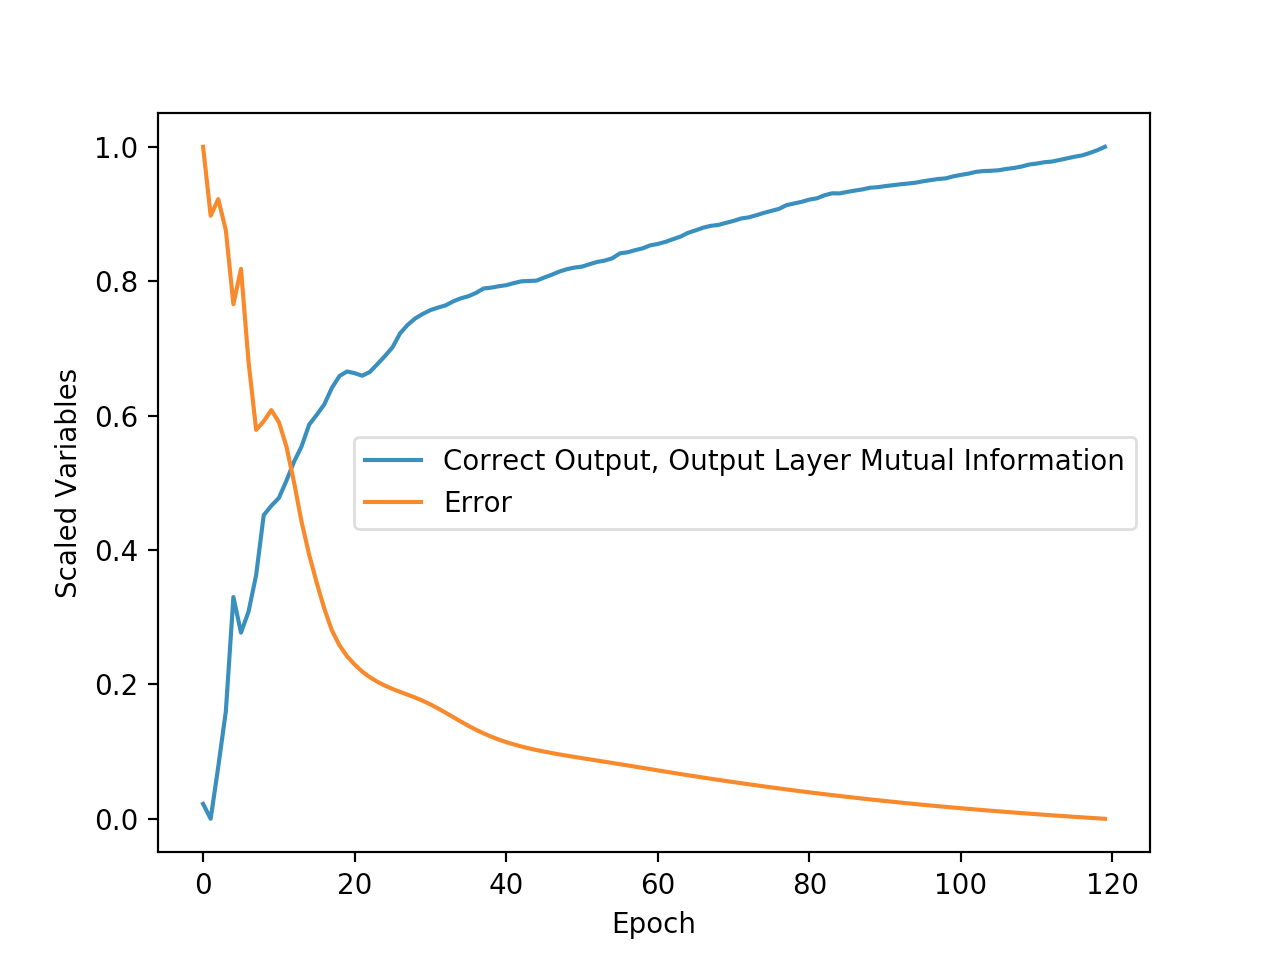
\includegraphics[width=\linewidth]{RNN_Images/25}
   
 However, this is not a useful indicator because it does not provide any information which is not just provided by the error. The mutual information between the hidden layer and the ground truth output has somewhat odd behavior during training (as shown in the previous section) and is therefore not necessarily a useful learning indicator. The mutual information of the hidden or output layer with the input, however, seems to be a very effective learning indicator. 
 
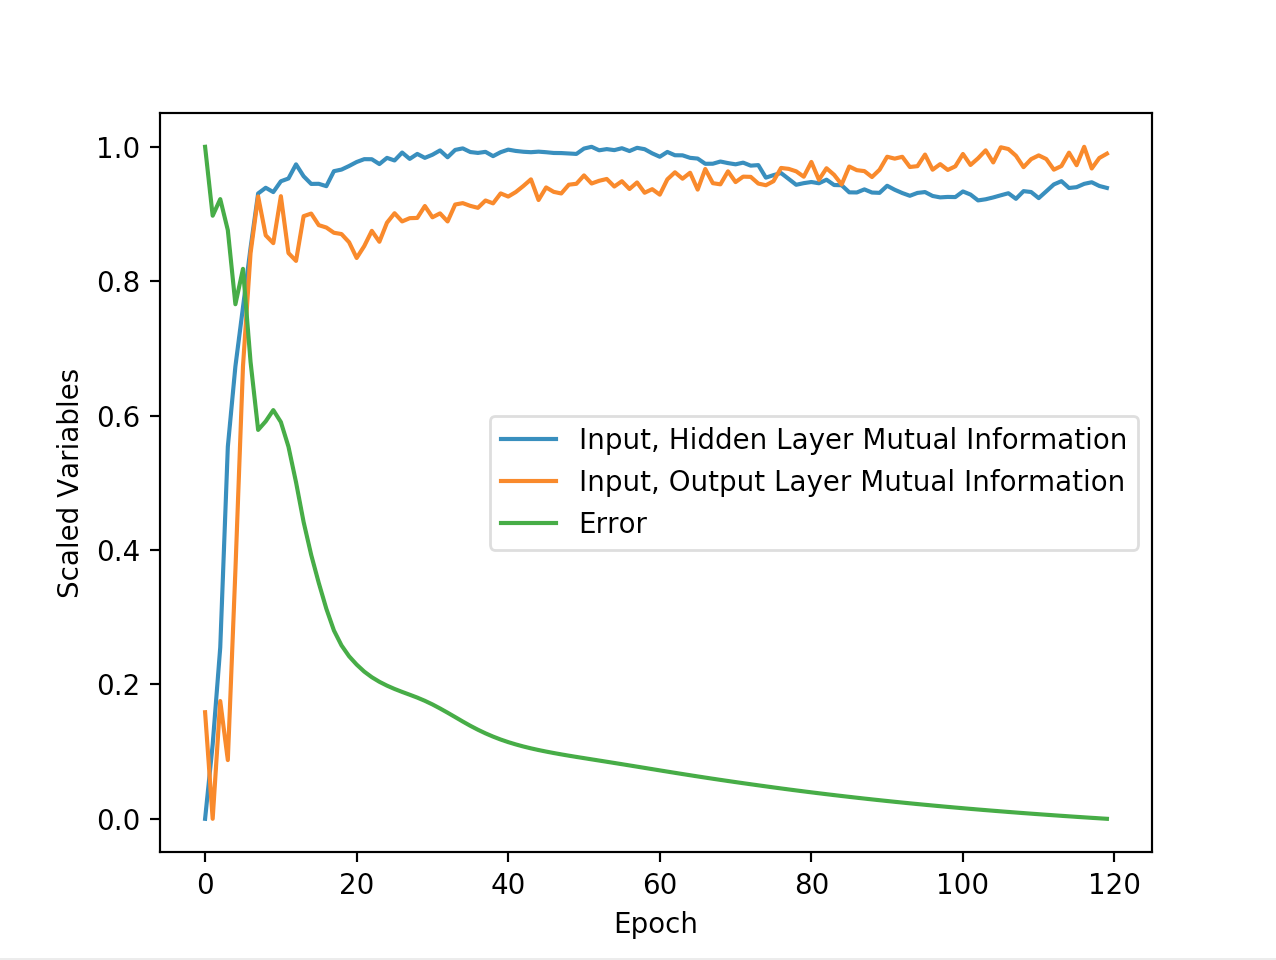
\includegraphics[width=\linewidth]{RNN_Images/21}
    
The above plot clearly shows the mutual information with the input increasing far faster than the error decreases. We also note that the mutual information between the input and the output is almost identical to the mutual information between the input and the hidden neurons. Therefore, clearly, they make equally good learning indicators. In addition to these mutual information measurements we found one other very effective learning indicator, TSE complexity. To calculate the TSE complexity in polynomial time, we approximated averages over all subsets of size k by averages over some randomly choose subset of the set of all subsets of size k. To ensure our approximation was valid, we tried varying the number of subsets chosen, and the results were altered only insignificantly. Not only was the TSE complexity a good learning indicator, but it also almost identically behaved like the mutual information with the input. The bellow plot shows this behavior. 
 
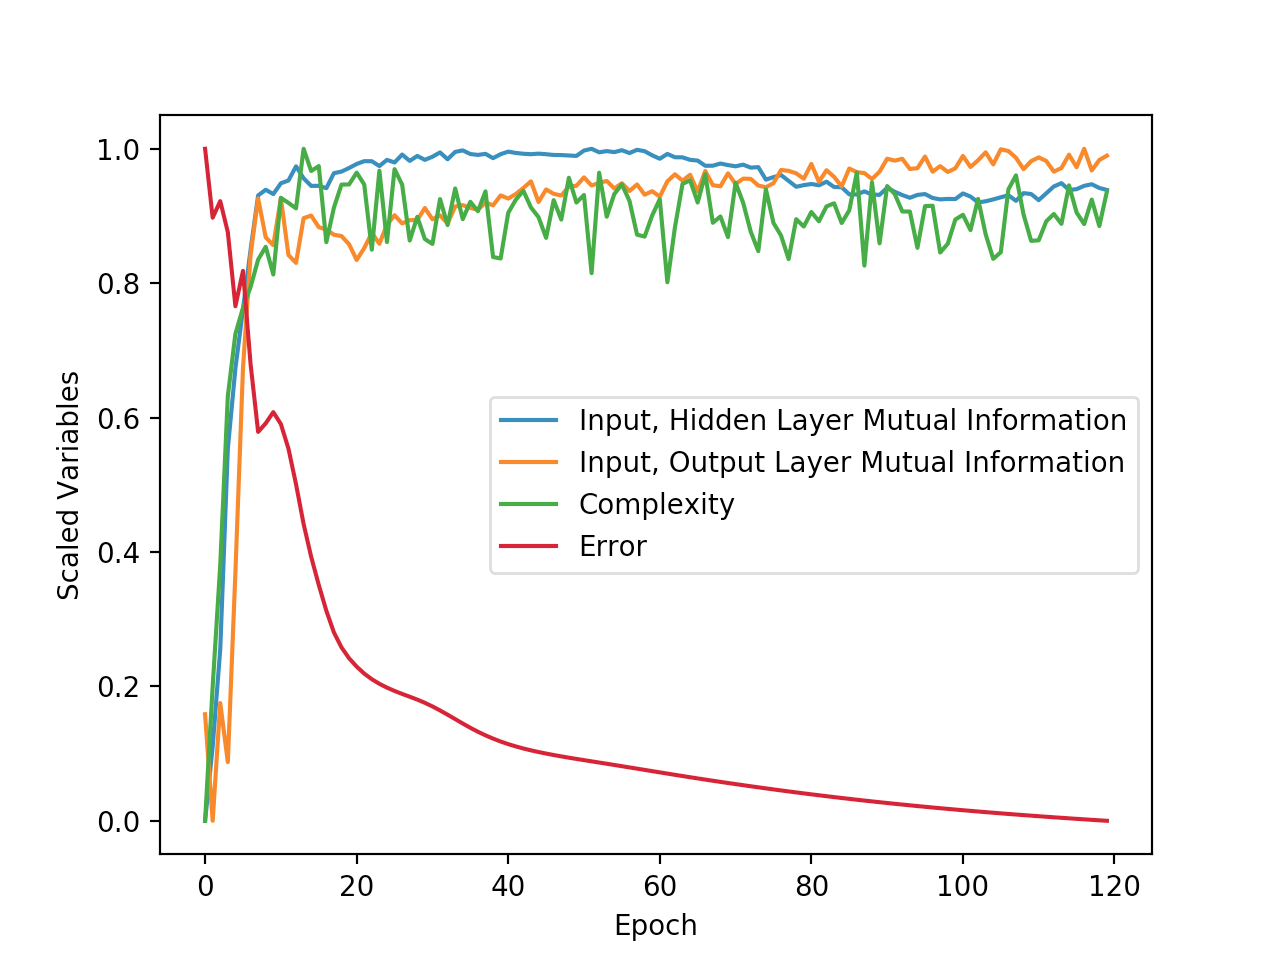
\includegraphics[width=\linewidth]{RNN_Images/19}
 
 \section{Analyzing the gradient}
 
 We analyzed how the mean the standard deviation of the gradient changes during training. As stated in "Opening the black box of Deep Neural Networks via Information" (if the information bottleneck principle applies) we should see two distinct phases to the gradients behavior. 
 
 [NOTE: I can not write anything about this until the gradient problem is fixed]
 
 \section{Conclusion}
 
 Fully recurrent neural networks have very chaotic and difficult to follow behavior. Analyzing information flow graphs is potentially a good way to understand the structure, however, they are rather difficult to interpret. Our ranking algorithm is potentially another useful tool, however, it is still difficult to interpret their results. Despite this, their results have been shown to fit what we would expect when it comes to showing the inputs have lower rank than the hidden neurons which have lower rank than the output. 
 
 Their is no indication that the information bottle neck principle applies to our fully recurrent neural network. However, it is still unknown weather this is a fluke of our neural network, or if the information bottleneck principle simply doesn't apply to fully recurrent neural networks. The mutual information between the output and the hidden neurons for our network behaves in an odd way during training that neither fits the information bottleneck principle nor the more basic idea of the mutual information always increasing. 
 
 [NOTE: We might have to change this if the gradient ends up showing information bottleneck like results once we fix it]
 
After training (during testing), the mutual information of neurons with the input is negatively correlated with the mutual information of neurons with the input. This most likly indicates that some neurons are more important than others, and that this effect overwhelms the fact that some neurons store more information about the input and some neurons store more information about the output. The idea of mutual information statistics being a useful indicator of learning certainly applies to fully recurrent neural networks. Specifically, the mutual information with the input and the TSE complexity are good learning indicators. 

\section{Future Work}

The obvious piece of future work is trying to re test hypothesis where we found negative results with other recurrent neural networks. This will indicate wether our negative results represent facts about recurrent neural networks, or are just flukes of our network. Specifically, it is important to test the information bottle neck principle on other recurrent neural networks. 

In my opinion, the most important and difficult piece of future work is finding a better way to analyze the information flow graph. I believe the information flow graph is a great starting point for analyzing recurrent neural networks. However, it is a difficult starting point simply due to the problem of understanding neural networks being a very difficult problem. It is unclear whether the information flow graph is truly random and chaotic, or if it is just very difficult to interpret. If the result is the former (which would surprise me), an additional piece of future work would be designing a new method of analyzing the way information flows in the network.

Another piece of future work is applying the ranking algorithm to larger networks, and applying more tests of the effectiveness of the ranking algorithm. Applying the ranking algorithm to larger networks could help should if their are patterns in the ranking. For example, if their are bands of neurons at different values (represented by spikes in the histogram) this could represent the natural development of "layer" like structures in a fully recurrent neural network. To further test the ranking algorithm, it could be applied to a feed forward neural network to see how well it mimics the desired results (having the rank of a neural be proportional to the layer that neuron is in). 

It would also be interesting to perform a more rigorous analysis of learning indicators. For example, one could analyze how the learning indicates behave under various situations where the network is not set up correctly (set up in a way in which it fill successfully learn). This could be used to see if learning indicators provide useful diagnostics for "debugging" neural networks. I believe the next step for learning indicators is showing how the network is learning (and revealing flaws in the learning) rather than just showing if the network is learning. 

\nocite{ntnu}
\nocite{black_box}
\nocite{weather}
\nocite{disentangling_representations}
\nocite{info_bottleneck}
\nocite{rnn_time_series}
\nocite{rnn_stocks}
\nocite{speech}
\nocite{text}
\nocite{mutual_info}
\nocite{content_transfer}
\nocite{social_media}

\bibliographystyle{unsrt}
\bibliography{references}

\end{document}
